\documentclass{report}
\usepackage{graphicx}
\graphicspath{ {} }
\usepackage[portuges]{babel}
\usepackage{hyperref}
\usepackage{listings}
\usepackage{url}
\usepackage{soul}
\usepackage{subcaption}
\parindent=0pt
\parskip=2pt

\usepackage{listings}
\usepackage{color}

\definecolor{dkgreen}{rgb}{0,0.6,0}
\definecolor{gray}{rgb}{0.5,0.5,0.5}
\definecolor{mauve}{rgb}{0.58,0,0.82}

\lstset{frame=tb,
  language=C++,
  aboveskip=3mm,
  belowskip=3mm,
  showstringspaces=false,
  columns=flexible,
  basicstyle={\scriptsize\ttfamily},
  numbers=none,
  numberstyle=\tiny\color{gray},
  keywordstyle=\color{blue},
  commentstyle=\color{dkgreen},
  stringstyle=\color{mauve},
  breaklines=true,
  breakatwhitespace=true,
  tabsize=2
}
\begin{document}

\title{Computa\c{c}\~ao Gr\'afica \\ \setlength{\baselineskip}{1.5\baselineskip} \textbf{Transforma\c{c}\~oes Geom\'etricas} \\ Relat\'orio de Desenvolvimento}
\author{ Jo\~ao Manuel Martins Cerqueira (A65432) \and S\'onia Catarina Guerra Costa (A71506) \and Tiago Costa Loureiro (A71191)}
\date{Ano letivo 2016/2017}

\begin{figure}
\centering
\includegraphics[scale=0.3]{logo_eeng.png}
\end{figure}



\maketitle 

\tableofcontents

% CAPITULO 1

\chapter{Introdu\c{c}\~{a}o}
 
Este trabalho pr\'atico incide-se no desenvolvimento de uma representa\c{c}\~ao est\'atica do sistema solar, incluindo o sol, os planetas e algumas das respetivas luas, atrav\'es de modelos dispostos hierarquimente, compostas por figuras e transforma\c{c}\~oes geom\'etricas definidas pr\'eviamente pelo utilizador. \\ Pretende-se que o programa leia a partir de um ficheiro $XML$ as transforma\c{c}\~oes geom\'etricas a fazer e os nomes dos ficheiros onde os pontos necess\'arios para construir os objetos est\~ao guardados e construa os mesmos. 

\section{Estrutura do documento}
A estrutura que este relat\'orio segue, excluindo o presente cap\'itulo onde se faz uma pequena introdu\c{c}\~{a}o do assunto, \'e: 
\begin{itemize}
\item No cap\'itulo 2 faz-se uma an\'alise detalhada do problema proposto especificando-se os par\^ametros de entrada do programa e os resultados obtidos.
\item No cap\'itulo 3 faz-se referencia \`a Conce\c{c}\~{a}o / Desenho da Resolu\c{c}\~{a}o dos problemas propostos, mostrando assim as estruturas de dados e todos os algoritmos usados durante a realiza\c{c}\~{a}o deste trabalho.
\item No cap\'itulo 4 faz-se refer\^encia a decis\~{o}es e problemas de implementa\c{c}\~{a}o que surgiram assim como os passos para executar o programa. 
\item No cap\'itulo 5 faz-se uma conclus\~{a}o / s\'intese de todo o trabalho realizado e uma an\'alise cr\'itica dos resultados.
\item No cap\'itulo 6 s\~ao feitas refer\^encias a fontes utilizadas durante a realiza\c{c}\~ao do trabalho.
\item Por \'ultimo, em ap\^endice encontra-se o c\'odigo necess\'ario para a implementa\c{c}\~{a}o do programa.
\end{itemize}


% CAPITULO 2
\chapter{An\'alise e Especifica\c{c}\~{a}o} 
\section{Especifica\c{c}\~{a}o do Problema} % 2.1
Neste trabalho pretende-se desenvolver um cen\'ario recorrendo a figuras e transforma\c{c}\~oes geom\'etricas obtidas pr\'eviamente atrav\'es da leitura de um ficheiro $XML$ cujo o nome \'e dado ao programa como argumento. Neste ficheiro est\~ao hierarquicamente definidos grupos, e subgrupos se aplic\'avel, que cont\^em a informa\c{c}\~ao necess\'aria para criar um cen\'ario em 3 dimens\~oes, nomeadamente os nomes dos ficheiros $.3d$ onde anteriormente foram guardados os v\'ertices correspondentes \`a cria\c{c}\~ao de cada figura. De seguida, aplicando as respetivas transforma\c{c}\~oes geom\'etricas, armazenadas tamb\'em aquando da leitura do $XML$, \'e gerada a figura final.
\begin{figure}[h]
\centering
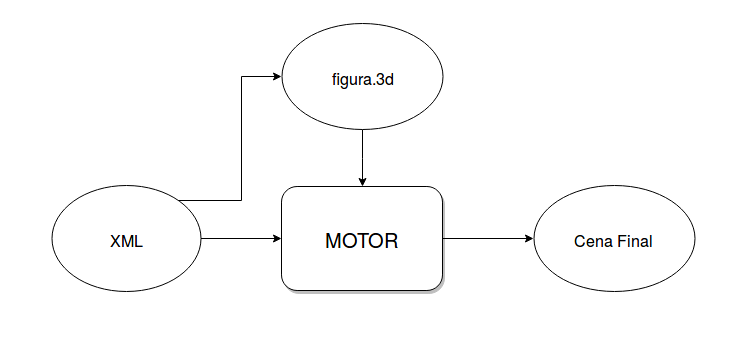
\includegraphics[scale=0.3]{diagrama.png}
\caption{Diagrama do trabalho}
\end{figure}


% CAPITULO 3
\chapter{Conce\c{c}\~{a}o/Desenho da Resolu\c{c}\~{a}o} 
%!!!!!!!!!!!!!!!!!!!!!!!!!!!!!!!!!!!!!!!!!!!!!!!!!!!!!!!!!!!!!!!!!!!!!!!!!!!!!!!!!!!!!!!!!!!!!!!!!!!!!!!!!!!!!!!!!!!!!!!!!!!!!!!!!!!!!!!!!!!!!!!!!!!!!!!!!!!!!!!!!!!!!!!!!!!!!!!!
\section{Leitura do XML} % 3.1 - 
Sabendo que o ficheiro $XML$ est\'a definido hierarquicamente por grupos, pretende ler-se as informa\c{c}\~oes referentes ao grupo pai e depois verificar se existe subgrupos. Cada grupo cont\'em o nome do ficheiro $.3d$ que ser\'a necess\'ario ler para construir a figura pedida e as suas transforma\c{c}\~oes geom\'etricas, podendo tamb\'em conter subgrupos. Estes subgrupos, se nada for dito, herdam as transforma\c{c}\~oes geom\'etricas do pai.
\\
Tentou manter-se a leitura do $XML$ simples mas eficaz. Foram utilizados ent\~ao dois ciclos, um para os grupos externos que neste caso s\~ao os planetas e estrelas, e outro para os grupos internos que representam as luas. Desta forma, consegue-se representar qualquer sistema solar.
Em cada um destes ciclos s\~ao lidos os 3 tipos de transorma\c{c}\~oes obtendo assim a posi\c{c}\~ao de cada planeta, estrela ou lua, sendo esta em relação \`a origem do referencial.
\\

\begin{lstlisting}[caption={Excerto do ficheiro solar.xml},captionpos=b]
    <group>
        <translate X="80" /> 
        <rotate angle="0" axisX="0" axisY="1" axisZ="0" />
        <scale X="4.5" Y="4.5" Z="4.5" /> <!-- terra -->

        <models>
            <model file="sphere.3d" />
        </models>

        <group>
            <translate Y="12" /> 
            <rotate angle="0" axisX="0" axisY="1" axisZ="0" />
            <scale X="1.2" Y="1.2" Z="1.2" /> <!-- lua  -->

            <models>
                <model file="sphere.3d" />
            </models>
        </group>
    </group>
\end{lstlisting}

\subsection{Estruturas de dados}
Os nomes dos ficheiros $.3d$ s\~ao guardados num vetor pela ordem em que s\~ao lidos, assim como as informa\c{c}\~oes relativas \'as transforma\c{c}\~oes geom\'etricas para que depois a leitura destas estruturas seja feita atrav\'es do \'indice respetivo.
Para mais f\'acil utiliza\c{c}\~ao de vetores, tendo em conta que se est\'a a trabalhar num sistema de eixos tridimensional, define-se como estrutura um vetor que recebe um tuplo de 3 floats. Desta forma, s\~ao armazenadas as transforma\c{c}\~oes geom\'etricas, escalas, transla\c{c}\~oes e rota\c{c}\~oes, no entanto nesta \'ultima, \'e necess\'ario criar um vetor de floats para guardar os \^angulos, pois a fun\c{c}\~ao $glRotatef$ recebe 4 argumentos. 
Esta estrutura foi tamb\'em utilizada para guardar cada cor referente aos astros do sistema solar pois, como \'e usado o sistema de cores RGB, s\~ao necess\'arios 3 valores para definir determinada cor.
\\

\begin{lstlisting}[caption={Estruturas de dados},captionpos=b]
//Estrutura para guardar 3 floats
    typedef vector< tuple<float, float, float> > vector3f;

// Vector que guarda a lista de ficheiros
    vector3f lista_translacoes;
    vector3f lista_escalas;
    vector3f lista_rotacoes;
    vector<float> lista_angulos;

// Vector que guarda o nome de todos os ficheiros
    vector<string> lista_ficheiros;

// Vector que guarda a lista das cores (1 para cada figura)
    vector3f lista_cores; 

\end{lstlisting}

\clearpage
\section{Leitura dos ficheiros .3d}
Percorrendo o vetor onde est\~ao armazenados os nomes dos ficheiros, como j\'a foi mencionado anteriormente, abre-se o respetivo ficheiro $.3d$. Se esta opera\c{c}\~ao n\~ao for conclu\'ida com sucesso, o programa termina com uma mensagem de erro. 
A primeira linha de cada ficheiro cont\'em o n\'umero de v\'ertices da figura, por isso essa linha \'e ignorada, as restantes linhas s\~ao lidas e os v\'ertices nelas contidos s\~ao armazenados numa estrutura do tipo $vector3f$, que foi mencionada no ponto anterior. Terminada a leitura de todas as linhas, o ficheiro \'e fechado e ap\'os terminar de construir esta figura, o vetor onde os v\'ertices foram guardados \'e limpo, para ser utilizado com o pr\'oximo ficheiro.
\\
\begin{lstlisting}[caption={Leitura dos ficheiros .3d},captionpos=b]
for (int i = 0; i <= lista_ficheiros.size()-1; ++i){

        const char *f = lista_ficheiros[i].c_str();
        ifstream fi(f);

        if (fi.is_open()){
            while(getline(fi, str)){ //ler todos os vertices
                //a primeira linha contem o numero de vertices, ignorar
                if(primeira_linha==0){ 
                    primeira_linha=1;
                } 
                else {
                    istringstream ss(str);
                    ss >> v1;
                    ss >> v2;
                    ss >> v3;
                    vertices.push_back(tuple<float,float,float>(v1,v2,v3));
                }
            }
            fi.close();
            primeira_linha = 0;
        }
        else{
            cerr << "Erro: Nao foi possivel abrir o ficheiro " << lista_ficheiros[i] << "." << endl;
            exit(1);
        }
(...)
        vertices.clear();
}
\end{lstlisting}

\clearpage
\section{Desenvolvimento das figuras}
Cada figura \'e gerada a partir da constru\c{c}\~ao sucessiva de tri\^angulos cujos v\'ertices foram pr\'eviamente guardados no vetor $vertices$. Primeiro, foram atribu\'idas as cores referentes a cada astro e em seguida aplicadas as respetivas transforma\c{c}\~oes, percorrendo os vetores correspondentes a cada informa\c{c}\~ao, dando de seguida \'inicio \`a constru\c{c}\~ao dos tri\^angulos.
Para que estas altera\c{c}\~oes n\~ao se acumulem, \'e feito um $glPushMatrix()$ antes e $glPopMatrix()$ depois de cada figura.
A representa\c{c}\~ao do sistema solar pode ser vista no modo $fill$, $point$ e $line$, para isso bastando clicar na imagem com o bot\~ao direito do rato para mudar o modo. 
\begin{lstlisting}[caption={Consctru\c{c}\~ao das figuras},captionpos=b]
    glPushMatrix();

        glColor3f(get<0>(lista_cores[i]), get<1>(lista_cores[i]), get<2>(lista_cores[i]));
            
        glTranslatef(get<0>(lista_translacoes[i]), get<1>(lista_translacoes[i]), get<2>(lista_translacoes[i]));
        glRotatef(lista_angulos[i], get<0>(lista_rotacoes[i]),get<1>(lista_rotacoes[i]),get<2>(lista_rotacoes[i]));
        glScalef(get<0>(lista_escalas[i]), get<1>(lista_escalas[i]),get<2>(lista_escalas[i]));
        
        glBegin(GL_TRIANGLES);
            for (int j = 0; j < vertices.size(); ++j){
                glVertex3f(get<0>(vertices[j]), get<1>(vertices[j]), get<2>(vertices[j]));
            }
        glEnd();

    glPopMatrix();
\end{lstlisting}

\begin{figure}[h]
\centering
\includegraphics[scale=0.3]{sistema_solar.png}
\caption{Representa\c{c}\~ao do Sistema Solar}
\end{figure}

\clearpage
% CAPITULO 5

\chapter{Conclus\~{a}o}
Pode-se concluir que a implementa\c{c}\~ao das transforma\c{c}\~oes geom\'etricas exigiu o uso de estruturas  de forma a conseguir gerir os dados e as transforma\c{c}\~oes. Houve alguma dificuldade ao decidir que tipo de estruturas usar e qual a estrat\'egia a ser aplicada de modo a tornar o programa mais r\'apido e eficiente. Contudo, a forma utilizada para ler os ficheiros ser\'a \'util na implementa\c{c}\~ao dos VBO's numa pr\'oxima fase.
Para que o programa seja de f\'acil acesso a qualquer utilizador, foi criada uma makefile que permite executar todo o programa desde o input at\'e \`a constru\c{c}\~ao final da representa\c{c}\~ao do sistema solar.
\clearpage
\chapter{Refer\^encias}

\begin{itemize}\newline

\item https://www.khronos.org/registry/OpenGL-Refpages/gl2.1/
\item http://stackoverflow.com/questions/170686/what-is-the-best-open-xml-parser-
for-c
\item http://www.cplusplus.com/doc/tutorial/files/
\item https://elearning.uminho.pt/


\end{itemize}
%%%%%%%%%%%%%%%%%%%%%%%%%%%%%%%%%%%%%%%%%%%%%%%%%%%%%%%%%%%%%%%%%%%%%%%%%%%%%%%%%%%%%%%%%%%%%%%%%%%%%%%
\appendix
\chapter{Ap\^endice}
\section{C\'odigo do Motor}
\begin{lstlisting}
#ifdef __APPLE__
#include <GLUT/glut.h>
#else
#include <GL/glut.h>
#endif

#include "tinyxml/tinyxml.h"
#define _USE_MATH_DEFINES
#include <math.h>
#include <vector>

#include <iostream>
#include <fstream>
#include <sstream>
#include <cstring>
#include <string>
#include <tuple>


 // para não estar sempre a escrever std::
 using namespace std;

//Estrutura para guardar 3 floats
typedef vector< tuple<float, float, float> > vector3f;

// Vector que guarda a lista de ficheiros
vector3f lista_translacoes;
vector3f lista_escalas;
vector3f lista_rotacoes;
vector<float> lista_angulos;

// Vector que guarda o nome de todos os ficheiros
vector<string> lista_ficheiros;

// Vector que guarda a lista das cores (1 para cada figura)
vector3f lista_cores; 

//variaveis de transformacoes usadas ao ler o XML
int translate_x = 0, translate_y = 0, translate_z = 0,
    scale_x = 1, scale_y = 1, scale_z = 1,
    angulo = 0, rotate_x = 0, rotate_y = 0, rotate_z = 0;
/* Ainda não é usado
#define EXP 0
#define FPS 1
*/

// flag para mudar o drwing mode
int flag_drawing_mode = 1; 

// ângulos para "rodar a camera" 
float alfa = 0.0f, beta = 0.0f, radius = 500.0f;
float camX = 0.0f, camY = 0.0f, camZ = 0.0f;

/* Ainda não é usado
float dx = 0.0f;
float dy = 0.0f;
float dz = 0.0f;
int modo_camera = 0;
 */

/* Esta função vai buscar os nomes dos ficheiros .3d que estão no vector lista_ficheiros
 * Desenha todos os pontos de cada ficheiro e por ficheiro atribui uma cor do vector lista_cores
 */

void definir_cores(){
    lista_cores.push_back(tuple<float,float,float>(1.0, 0.94, 0.0)); //sol
    lista_cores.push_back(tuple<float,float,float>(0.87, 0.72, 0.53)); //mercurio
    lista_cores.push_back(tuple<float,float,float>(0.82, 0.41, 0.12)); //venus
    lista_cores.push_back(tuple<float,float,float>(0.29, 0.59, 0.82)); //terra
    lista_cores.push_back(tuple<float,float,float>(0.97, 0.91, 0.81)); //lua
    lista_cores.push_back(tuple<float,float,float>(0.76, 0.23, 0.13)); //marte
    lista_cores.push_back(tuple<float,float,float>(0.97, 0.91, 0.56)); //jupiter
    lista_cores.push_back(tuple<float,float,float>(0.57, 0.64, 0.69)); //lua
    lista_cores.push_back(tuple<float,float,float>(0.83, 0.69, 0.22)); //lua
    lista_cores.push_back(tuple<float,float,float>(0.66, 0.6, 0.53)); //lua
    lista_cores.push_back(tuple<float,float,float>(0.4, 0.22, 0.33)); //lua
    lista_cores.push_back(tuple<float,float,float>(0.9, 0.67, 0.44)); //saturno
    lista_cores.push_back(tuple<float,float,float>(0.76, 0.6, 0.42)); //lua
    lista_cores.push_back(tuple<float,float,float>(0.76, 0.6, 0.42)); //lua
    lista_cores.push_back(tuple<float,float,float>(0.49, 0.98, 1.0)); //urano
    lista_cores.push_back(tuple<float,float,float>(0.0, 0.0, 0.61)); //neptuno
    lista_cores.push_back(tuple<float,float,float>(0.97, 0.91, 0.81)); //lua    
}

void desenha(){
    /*
    * Variaveis
    */
    vector3f vertices;  //vector< tuple<float, float, float> >
    float v1 = 0, v2=0, v3=0;
    string str;
    int primeira_linha = 0;
    
    /*
    * percorrer lista com o nome dos ficheiros
    */
    
    for (int i = 0; i <= lista_ficheiros.size()-1; ++i){

        const char *f = lista_ficheiros[i].c_str();
        
        ifstream fi(f);

        if (fi.is_open()){
            while(getline(fi, str)){ //ler todos os vertices
                //a primeira linha contem o numero de vertices, passa a frente
                if(primeira_linha==0){ 
                    primeira_linha=1;
                } 
                else {
                    istringstream ss(str);
                    ss >> v1;
                    ss >> v2;
                    ss >> v3;
                    
                    vertices.push_back(tuple<float,float,float>(v1,v2,v3));
                }
            }
            fi.close();
            primeira_linha = 0;
        }
        else{
            cerr << "Erro: Não foi possível abrir o ficheiro " << lista_ficheiros[i] << "." << endl;
            exit(1);
        }

        /*
        * desenhar objeto
        */

        definir_cores();

        glPushMatrix();

            glColor3f(get<0>(lista_cores[i]), get<1>(lista_cores[i]), get<2>(lista_cores[i]));
            
            glTranslatef(get<0>(lista_translacoes[i]), get<1>(lista_translacoes[i]), get<2>(lista_translacoes[i]));
            glRotatef(lista_angulos[i], get<0>(lista_rotacoes[i]),get<1>(lista_rotacoes[i]),get<2>(lista_rotacoes[i]));
            glScalef(get<0>(lista_escalas[i]), get<1>(lista_escalas[i]),get<2>(lista_escalas[i]));
            
            glBegin(GL_TRIANGLES);
                for (int j = 0; j < vertices.size(); ++j){
                    glVertex3f(get<0>(vertices[j]), get<1>(vertices[j]), get<2>(vertices[j]));
                }
            glEnd();

        glPopMatrix();
        
        
        /*
        * clear vector for next file
        */
        vertices.clear();

    }
}

void spherical2Cartesian() {

    camX = radius * cos(beta) * sin(alfa);
    camY = radius * sin(beta);
    camZ = radius * cos(beta) * cos(alfa);
}

void changeSize(int w, int h) {

    // Prevent a divide by zero, when window is too short
    // (you cant make a window with zero width).
    if(h == 0)
        h = 1;

    // compute window's aspect ratio
    float ratio = w * 1.0 / h;

    // Set the projection matrix as current
    glMatrixMode(GL_PROJECTION);
    // Load Identity Matrix
    glLoadIdentity();

    // Set the viewport to be the entire window
    glViewport(0, 0, w, h);

    // Set perspective
    gluPerspective(45.0f ,ratio, 1.0f ,1000.0f);

    // return to the model view matrix mode
    glMatrixMode(GL_MODELVIEW);
}


void renderScene(void) {

    // clear buffers
    glClear(GL_COLOR_BUFFER_BIT | GL_DEPTH_BUFFER_BIT);

    // set the camera
    glLoadIdentity();
    /*//visao lateral dos planetas
    gluLookAt(300, 0, 1000,
              300.0f, 0.0f, 0.0f,
              0.0f, 1.0f, 0.0f);
    */    

    gluLookAt(camX, camY, camZ,
              250.0f, 50.0f, 50.0f,
              0.0f, 1.0f, 0.0f);

    // put the geometric transformations here
    if(flag_drawing_mode == 0){
        glPolygonMode(GL_FRONT_AND_BACK,GL_FILL);
    }else if(flag_drawing_mode == 1){
        glPolygonMode(GL_FRONT_AND_BACK,GL_LINE);
    }else if(flag_drawing_mode == 2){
        glPolygonMode(GL_FRONT_AND_BACK,GL_POINT);
    }

    //glutWireTeapot(1);
    desenha(); 

    // End of frame
    glutSwapBuffers();
}


void processKeys(unsigned char c, int xx, int yy) {

}


void processSpecialKeys(int key, int xx, int yy) {

    switch (key) {
        case GLUT_KEY_RIGHT:
            alfa -= 0.1; break;

        case GLUT_KEY_LEFT:
            alfa += 0.1; break;

        case GLUT_KEY_UP:
            beta += 0.1f;
            if (beta > 1.5f)
                beta = 1.5f;
            break;

        case GLUT_KEY_DOWN:
            beta -= 0.1f;
            if (beta < -1.5f)
                beta = -1.5f;
            break;

        case GLUT_KEY_PAGE_UP:
            radius -= 0.1f;
            if (radius < 0.1f)
                radius = 0.1f;
            break;

        case GLUT_KEY_PAGE_DOWN:
            radius += 0.1f;
            break;
    }
    spherical2Cartesian();
    glutPostRedisplay();

}


int translacao(TiXmlElement* translate){
    
    const char *aux_x = translate->Attribute("X");
    const char *aux_y = translate->Attribute("Y");
    const char *aux_z = translate->Attribute("Z");

    if(aux_x)   translate_x = atoi(aux_x);
    if(aux_y)   translate_y = atof(aux_y);
    if(aux_z)   translate_z = atof(aux_z);

}
int rotacao(TiXmlElement* rotate){
    
    const char *aux_a = rotate->Attribute("angle");
    const char *aux_x = rotate->Attribute("axisX");
    const char *aux_y = rotate->Attribute("axisY");
    const char *aux_z = rotate->Attribute("axisZ");

    if(aux_a)   angulo = atof(aux_a);
    if(aux_x)   rotate_x = atof(aux_x);
    if(aux_y)   rotate_y = atof(aux_y);
    if(aux_z)   rotate_z = atof(aux_z);

}
int escala(TiXmlElement* scale){

    const char *aux_x = scale->Attribute("X");
    const char *aux_y = scale->Attribute("Y");
    const char *aux_z = scale->Attribute("Z");

    if(aux_x)   scale_x = atof(scale->Attribute("X"));
    if(aux_y)   scale_y = atof(scale->Attribute("Y"));
    if(aux_z)   scale_z = atof(scale->Attribute("Z"));

}
int modelo(){}


int le_xml(char *nome){
    int erros = 0;
    string caminho = "xml/" + (string)nome;

    TiXmlDocument doc;


    if(!doc.LoadFile(caminho.c_str()) ){
        cout << "Nome do ficheiro inválido" << caminho << endl;
        return erros+1;
    }

    //scene
    TiXmlElement* raiz = doc.FirstChildElement();
    if(raiz == NULL) return erros+1;

    // Grupos
    TiXmlElement* grupo_ext = NULL;
    for(grupo_ext=raiz->FirstChildElement("group"); grupo_ext; grupo_ext=grupo_ext->NextSiblingElement("group")) {

        // TRANSLATE
        TiXmlElement* translate = grupo_ext->FirstChildElement("translate");
        if(translate != NULL)
            translacao(translate);

        // ROTATE
        TiXmlElement* rotate = grupo_ext->FirstChildElement("rotate");
        if(rotate != NULL)
            rotacao(rotate);

        // SCALE
        TiXmlElement* scale = grupo_ext->FirstChildElement("scale");
        if(scale != NULL)
            escala(scale);

        TiXmlElement* models = grupo_ext->FirstChildElement("models");
        if(models != NULL){
            const char* nome_aux = NULL;

            nome_aux = models->FirstChildElement("model")->Attribute("file");
            if (nome_aux == NULL) return 0;
            std::string nome_ficheiro = "";
            nome_ficheiro += nome_aux;

            lista_ficheiros.push_back(nome_ficheiro);
            lista_rotacoes.push_back(tuple<float,float,float>(rotate_x,rotate_y,rotate_z));
            lista_angulos.push_back(angulo);
            lista_translacoes.push_back(tuple<float,float,float>(translate_x,translate_y,translate_z));
            lista_escalas.push_back(tuple<float,float,float>(scale_x,scale_y,scale_z));

        }

        TiXmlElement* grupo_int = NULL;
        for(grupo_int=grupo_ext->FirstChildElement("group"); grupo_int; grupo_int=grupo_int->NextSiblingElement("group")) {
            // TRANSLATE
            TiXmlElement* translate = grupo_int->FirstChildElement("translate");
            if(translate != NULL)
                translacao(translate);

            // ROTATE
            TiXmlElement* rotate = grupo_int->FirstChildElement("rotate");
            if(rotate != NULL)
                rotacao(rotate);

            // ROTATE
            TiXmlElement* scale = grupo_int->FirstChildElement("scale");
            if(scale != NULL)
                escala(scale);

            TiXmlElement* models = grupo_int->FirstChildElement("models");
            if(models != NULL){
                const char* nome_aux = NULL;

                nome_aux = models->FirstChildElement("model")->Attribute("file");
                if (nome_aux == NULL) return 0;
                std::string nome_ficheiro = "";
                nome_ficheiro += nome_aux;

                lista_ficheiros.push_back(nome_ficheiro);
                lista_rotacoes.push_back(tuple<float,float,float>(rotate_x,rotate_y,rotate_z));
                lista_angulos.push_back(angulo);
                lista_translacoes.push_back(tuple<float,float,float>(translate_x,translate_y,translate_z));
                lista_escalas.push_back(tuple<float,float,float>(scale_x,scale_y,scale_z));

            }
        }
    }

    return 0;
}


void processMenuEvents(int option) {

    switch (option) {
        case 0 :
            flag_drawing_mode = 0;
            break;
        case 1 :
            flag_drawing_mode = 1;
            break;
        case 2 :
            flag_drawing_mode = 2;
            break;
        default:
            break;
    }

    glutPostRedisplay();

}

void createGLUTMenus() {

    int menu;

    menu = glutCreateMenu(processMenuEvents);

    glutAddMenuEntry("Fill",0);
    glutAddMenuEntry("Line",1);
    glutAddMenuEntry("Point",2);

    glutAttachMenu(GLUT_RIGHT_BUTTON);
}

int main(int argc, char **argv) {

// init GLUT and the window
    glutInit(&argc, argv);
    glutInitDisplayMode(GLUT_DEPTH|GLUT_DOUBLE|GLUT_RGBA);
    glutInitWindowPosition(0,0);
    glutInitWindowSize(glutGet(GLUT_SCREEN_WIDTH),glutGet(GLUT_SCREEN_HEIGHT));
    glutCreateWindow("MOTOR");

// Required callback registry
    glutDisplayFunc(renderScene);
    glutReshapeFunc(changeSize);

// Callback registration for keyboard processing
    glutKeyboardFunc(processKeys);
    glutSpecialFunc(processSpecialKeys);

// MENUS
    glutDetachMenu(GLUT_RIGHT_BUTTON);
    createGLUTMenus();


//  OpenGL settings
    glEnable(GL_DEPTH_TEST);
    glEnable(GL_CULL_FACE);

    glClearColor(1,1,1,1);

    le_xml(argv[1]);

    glutPostRedisplay();
    spherical2Cartesian();

// enter GLUT's main cycle
    glutMainLoop();

    return 0;
}

\end{lstlisting}
\clearpage
\section{Ficheiro solarf.xml}
\begin{lstlisting}
<?xml version="1.0" encoding="UTF-8" ?>
<scene>
    
    <group>
        <scale X="300" Y="500" Z="500" /> <!-- sol -->
        <translate X="-590" />
        <models>
            <model file="sphere.3d" />
        </models>
    </group> 

    <group>
        <translate X="28" /> 
        <rotate angle="15" axisX="0" axisY="1" axisZ="0" />
        <scale X="1.7" Y="1.7" Z="1.7" /> <!-- mercurio -->

        <models>
            <model file="sphere.3d" />
        </models>
    </group>

    <group>
        <translate X="50" /> 
        <rotate angle="30" axisX="0" axisY="1" axisZ="0" />
        <scale X="4.3" Y="4.3" Z="4.3" /> <!-- venus -->

        <models>
            <model file="sphere.3d" />
        </models>
    </group>

    <group>
        <translate X="80" /> 
        <rotate angle="0" axisX="0" axisY="1" axisZ="0" />
        <scale X="4.5" Y="4.5" Z="4.5" /> <!-- terra -->

        <models>
            <model file="sphere.3d" />
        </models>

        <group>
            <translate Y="12" /> 
            <rotate angle="0" axisX="0" axisY="1" axisZ="0" />
            <scale X="1.2" Y="1.2" Z="1.2" /> <!-- lua  -->

            <models>
                <model file="sphere.3d" />
            </models>
        </group>
    </group>

    <group>
        <translate X="100" Y="0" Z="0"/> 
        <rotate angle="75" axisX="0" axisY="1" axisZ="0" />
        <scale X="2.4" Y="2.4" Z="2.4" /> <!-- marte -->

        <models>
            <model file="sphere.3d" />
        </models>
    </group>

    <group>
        <translate X="230" /> 
        <rotate angle="90" axisX="0" axisY="1" axisZ="0" />
        <scale X="50.1" Y="50.1" Z="50.1" /> <!-- jupiter -->

        <models>
            <model file="sphere.3d" />
        </models>

        <group>
            <translate Y="50" Z="130"/> 
            <rotate angle="15" axisX="0" axisY="1" axisZ="0" />
            <scale X="1.2" Y="1.2" Z="1.2" /> <!-- lua europa -->

            <models>
                <model file="sphere.3d" />
            </models>
        </group>

        <group>
            <translate Y="130" Z ="90"/> 
            <rotate angle="30" axisX="0" axisY="1" axisZ="0" />
            <scale X="1.2" Y="1.2" Z="1.2" /> <!-- lua IO -->

            <models>
                <model file="sphere.3d" />
            </models>
        </group>

        <group>
            <translate Y="90" Z="140"/> 
            <rotate angle="45" axisX="0" axisY="1" axisZ="0" />
            <scale X="1.5" Y="1.5" Z="1.5" /> <!-- lua Ganimedes -->

            <models>
                <model file="sphere.3d" />
            </models>
        </group>

        <group>
            <translate Y="100" Z="130"/> 
            <rotate angle="60" axisX="0" axisY="1" axisZ="0" />
            <scale X="1.5" Y="1.5" Z="1.5" /> <!--lua calisto-->

            <models>
                <model file="sphere.3d" />
            </models>
        </group>
    </group>

    <group>
        <translate X="500" Y="0" Z="0"/> 
        <rotate angle="45" axisX="0" axisY="1" axisZ="0" />
        <scale X="42" Y="42" Z="42" /> <!-- saturno -->

        <models>
            <model file="sphere.3d" />
        </models>

        <group>
            
            <rotate angle="30" axisX="0" axisY="1" axisZ="1" />
            <scale X="60" Y="1.5" Z="60" /> <!-- anel -->

            <models>
                <model file="sphere.3d" />
            </models>
        </group>

        <group>
            <translate Y="100" /> 
            <rotate angle="120" axisX="0" axisY="1" axisZ="0" />
            <scale X="1.5" Y="1.5" Z="1.5" /> <!-- lua tita -->

            <models>
                <model file="sphere.3d" />
            </models>
        </group>


    </group>

    <group>
        <translate X="702" Y="0" Z="0"/> 
        <rotate angle="135" axisX="0" axisY="1" axisZ="0" />
        <scale X="16.8" Y="16.8" Z="16.8" /> <!-- urano -->
        <models>                        
            <model file="sphere.3d" />
        </models>
        
    </group>

    <group>
        <translate X="800" Y="0" Z="0"/> 
        <rotate angle="150" axisX="0" axisY="1" axisZ="0" />
        <scale X="16.3" Y="16.3" Z="16.3" /> <!-- neptuno -->

        <models>
            <model file="sphere.3d" />
        </models>

        <group>
            <translate Y="60" /> 
            <rotate angle="165" axisX="0" axisY="1" axisZ="0" />
            <scale X="1.1" Y="1.1" Z="1.1" /> <!-- lua tritao -->

            <models>
                <model file="sphere.3d" />
            </models>
        </group>
    </group>
</scene>


\end{lstlisting}


\end{document}